% ==============================================================================
%
%                                    DV017A
%                        Inledande Programmering i Java
%                                Laboration #2
%
% Author:   Jonas Sjöberg
%           Högskolan i Gävle
%           tel12jsg@student.hig.se
%           https://github.com/jonasjberg
%
% License:  Creative Commons Attribution-NonCommercial-ShareAlike 4.0
%           International.  See LICENSE.md for full licensing information.
% ==============================================================================

\documentclass[11pt,a4paper]{article}

\usepackage[utf8]{inputenc}
\inputencoding{utf8}
\usepackage[swedish]{babel}
\usepackage[T1]{fontenc}
\usepackage{lmodern}
\usepackage{fullpage}

\usepackage{textcomp}
\usepackage{url}
\usepackage{graphicx}

\usepackage{minted}
%\usemintedstyle{pastie}
\usemintedstyle{bw}

\usepackage{verbatim}
\usepackage{listings}

\usepackage{natbib}


\title{DV017A \\ Java-programmering \\ Laboration 2}

\author{\\
  Jonas Sjöberg\\
  860224\\
  Högskolan i Gävle,\\
  Elektronikingenjörsprogrammet,\\
  \texttt{tel12jsg@tudent.hig.se}
}

\date{}

\begin{document}
    \maketitle

    \begin{center}
    \begin{tabular}{l r}
        Datum: & Juni 2015 \\
        Kursansvarig lärare: & Atique Ullah
    \end{tabular}
    \end{center}

    \begin{abstract}
        Laboration i DV017A - Inledande programmering i Java.
        TODO: Utveckla abstrakt.
    \end{abstract}

    \newpage
    %\hypersetup{linkcolor=black}
    \setcounter{tocdepth}{3}
    \tableofcontents
    \newpage

    \section{Introduction}\label{sec:intro}
% TODO: Eventuell övergripande introduktion.


    \section{Uppgift 1}\label{sec:uppg01}

\subsection{Instruktioner}
\begin{verbatim}
1. Vad är det för speciellt med en konstant variabel och visa hur man
   deklarerar en sådan? Skriv ett litet program på några rader där du använder
   dig av en konstant variabel.
\end{verbatim}


\subsection{Lösning}
\subsubsection{Funktion}
% TODO: Eventuell beskrivning av #01 funktionalitet.

\subsubsection{Kommentar}

\quote{A final variable may only be assigned to once. Declaring a variable
final can serve as useful documentation that its value will not change and can
help avoid programming errors.}
%\cite{jle:static}

%Final variables
%http://docs.oracle.com/javase/specs/jls/se7/html/jls-4.html#jls-4.12.4
%The Java® Language Specification
%Java SE 7 Edition


\subsubsection{Källkod}
\javacode{src/main/Lab2Uppg01.java}
\label{src:uppg01}


\subsubsection{Skärmdump}
\begin{figure}[htbp]
    \centering
        
\includegraphics[width=\linewidth]{img/01.png}
    \caption{Körning av koden till Uppgift~\ref{sec:uppg01}}
\label{fig:uppg01-screenshot}
\end{figure}
% TODO: Lägg till skärmdump av #01.


%   \section{Uppgift 2}\label{sec:uppg02}

\subsection{Instruktioner}
\begin{verbatim}
2. Vilket värde får variablerna x och y efter det att uttrycket (a-g) beräknats
   (varje uttryck ska beräknas enskilt). Lös gärna först uppgiften i huvudet
   (lär man sig mycket på) utan att testa med något program.
   Följande deklaration finns i programmen:

       int x=4;
       int y=2;

       a.  y=x++;
       b.  y=++x;
       c.  y\*=x;
       d.  y+=(x+2);
       e.  y+=--x;
       f.  y+=x++
       g.  x=-y;
\end{verbatim}

\subsection{Lösning}
Lösningen av Uppgift \ref{sec:uppg02} använder en metod
\texttt{shotResults(String label)} för att skriva ut värdet av variablerna
\texttt{x} och \texttt{y} efter att varje uttryck beräknas.

\subsubsection{Funktion}

\subsubsection{Kommentar}

%                                  |  värde efter uttryck  |
%  uttryck  |      operation       |  int x      int y     |
% ==========|======================|=======================|
% (start)   |                      |      4          2     |
%     (A)   |    y    =    x++     |      5          4     |
%     (B)   |    y    =  ++x       |      6          6     |
%     (C)   |    y   *=    x       |      6          36    |
%     (D)   |    y   +=   (x + 2)  |      6          44    |
%     (E)   |    y   +=  --x       |      5          49    |
%     (F)   |    y   +=    x++     |      6          54    |
%     (G)   |    x    =   -y;      |     -54         54    |
%


\subsubsection{Källkod}
\inputminted[linenos]{java}{src/Lab2Uppg02.java}
\caption{Lab2Uppg02.java}
\label{src:uppg02}


\subsubsection{Skärmdump}
\begin{figure}[htbp]
    \centering
        
\includegraphics[width=\linewidth]{img/02.png}
    \caption{Körning av koden till Uppgift \ref{sec:uppg02}}
    \label{fig:uppg02-screenshot}
\end{figure}
% TODO: Lägg till skärmdump av #02.


%   \section{Uppgift 3}\label{sec:uppg#03}

\subsection{Instruktioner}
% TODO: Lägg till instruktioner för #03.


\subsection{Lösning}
\subsubsection{Funktion}
% TODO: Eventuell beskrivning av #03 funktionalitet.

\subsubsection{Kommentar}
% TODO: Eventuell kommentar på #03.


\subsubsection{Källkod}
\inputminted[linenos]{java}{src/Lab2Uppg#03.java}
\caption{Lab2Uppg#03.java}
\label{src:uppg#03}
% TODO: Lägg till källkod för #03.


\subsubsection{Skärmdump}
\begin{figure}[htbp]
    \centering
        \includegraphics[width=\linewidth]{img/#03.png}
    \caption{Körning av koden till Uppgift \ref{sec:uppg#03}}
    \label{fig:uppg#03-screenshot}
\end{figure}
% TODO: Lägg till skärmdump av #03.


%   \section{Uppgift 4}\label{sec:uppg04}

\subsection{Instruktioner}
\begin{verbatim}
4. Skriv programmet som spelar det klassiska gissa-talet spelet.  Programmet
   ska först slumpa ut ett tal mellan 1 och 100. Detta tal ska den som spelar
   klura ut. Om man gissat för lågt eller för högt så ska "Du har gissat för
   lågt!" resp "Du har gissat för högt!" skrivas ut på skärmen. Man ska få
   fortsätta gissa tills man gissat rätt, "Rätt gissat!" skrivs då ut. Även
   antal gissningar ska skrivas ut. Varje gång man gissat rätt ska man få välja
   om man vill spela spelet igen eller avsluta.
   Så här kan exempelvis en körning se ut:

        Välkommen till gissa-talet spelet!
        Du ska gissa på ett tal mellan 1 och 100
        gissa\> *75*
        Du har gissat för högt!
        gissa\> *35*
        Du har gissat för lågt!
        gissa\> *60*
        Du har gissat för högt!
        gissa\> *40*
        Rätt gissat! Du har gissat 4 gånger.
        Spela en gång till (j/n): *n*
        Adjö!
\end{verbatim}


\subsection{Lösning}
\subsubsection{Funktion}
% TODO: Eventuell beskrivning av #04 funktionalitet.

\subsubsection{Kommentar}
% TODO: Eventuell kommentar på #04.


\subsubsection{Källkod}
%\inputminted[linenos]{java}{src/main/Lab2Uppg04.java}
\javacode{src/main/Lab2Uppg04.java}
%\caption{Lab2Uppg04.java}
\label{src:uppg04}


\subsubsection{Skärmdump}
\begin{figure}[htbp]
    \centering
        
\includegraphics[width=\linewidth]{img/04.png}
    \caption{Körning av koden till Uppgift~\ref{sec:uppg04}}
    \label{fig:uppg04-screenshot}
\end{figure}
% TODO: Lägg till skärmdump av #04.


%   \section{Uppgift 5}\label{sec:uppg05}

\subsection{Instruktioner}
% TODO: Lägg till instruktioner för #05.


\subsection{Lösning}
\subsubsection{Funktion}
% TODO: Eventuell beskrivning av #05 funktionalitet.

\subsubsection{Kommentar}
% TODO: Eventuell kommentar på #05.


\subsubsection{Källkod}
\inputminted[linenos]{java}{src/Lab2Uppg05.java}
\caption{Lab2Uppg05.java}
\label{src:uppg05}
% TODO: Lägg till källkod för #05.


\subsubsection{Skärmdump}
\begin{figure}[htbp]
    \centering
        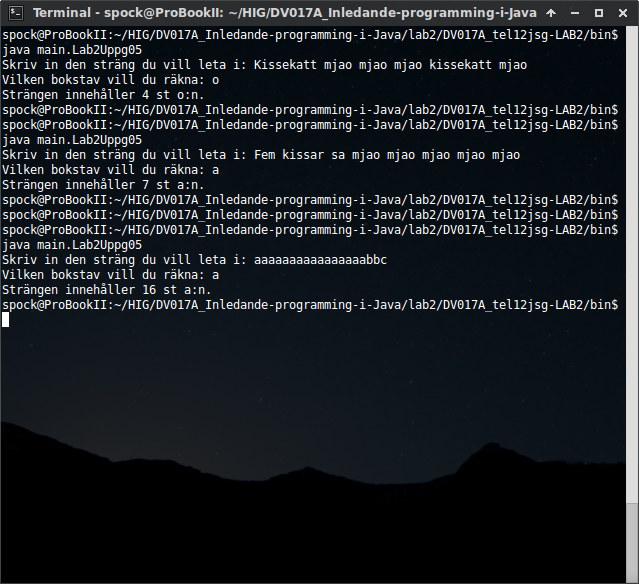
\includegraphics[width=\linewidth]{img/05.png}
    \caption{Körning av koden till Uppgift \ref{sec:uppg05}}
    \label{fig:uppg05-screenshot}
\end{figure}
% TODO: Lägg till skärmdump av #05.


%   \section{Uppgift 6}\label{sec:uppg06}

\subsection{Instruktioner}
\begin{verbatim}
6. Skriv ett program som räknar och skriver ut hur många förekomster det finns
   av vokalerna a, e, i, o, u och y i en sträng. Strängen ska matas in av den
   som kör programmet. Du ska deklarera en räknar-variabel för varje vokal och
   använda dig av en switch-sats.
   Exempel på körning:

        Mata in strängen: *Du har min kursbok*
        I strängen finns: 1 st a:n
        0 st e:n
        1 st i:n
        1 st o:n
        2 st u:n
        0 st y:n
\end{verbatim}


\subsection{Lösning}
\subsubsection{Funktion}
% TODO: Eventuell beskrivning av #06 funktionalitet.

\subsubsection{Kommentar}
% TODO: Eventuell kommentar på #06.


\subsubsection{Källkod}
\javacode{src/main/Lab2Uppg06.java}
%\caption{Lab2Uppg06.java}
\label{src:uppg06}


\subsubsection{Skärmdump}
\begin{figure}[htbp]
    \centering
        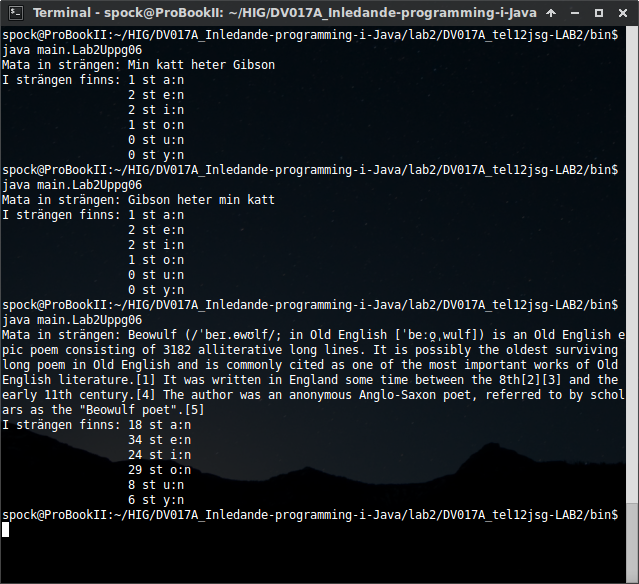
\includegraphics[width=\linewidth]{img/06.png}
    \caption{Körning av koden till Uppgift~\ref{sec:uppg06}}
    \label{fig:uppg06-screenshot}
\end{figure}
% TODO: Lägg till skärmdump av #06.


%   \section{Uppgift 7}\label{sec:uppg07}

\subsection{Instruktioner}
\begin{verbatim}
7. Ett heltal är ett primtal om det bara är delbart med 1 och sig självt.
   Exempelvis så är 2, 3, 5 och 7 primtal, men 4, 6, 8 och 9 är ej primtal.
   Skriv ett program som kontrollerar och skriver ut om ett tal är primtal
   eller ej. Den som kör programmet ska skriva in talet.
   Tips: använd modulus-operatorn %.
\end{verbatim}


\subsection{Lösning}

\subsubsection{Källkod}
\javacode{src/main/Lab2Uppg07.java}
\caption{Lab2Uppg07.java}
\label{src:uppg07}


\subsubsection{Skärmdump}
\begin{figure}[htbp]
    \centering
        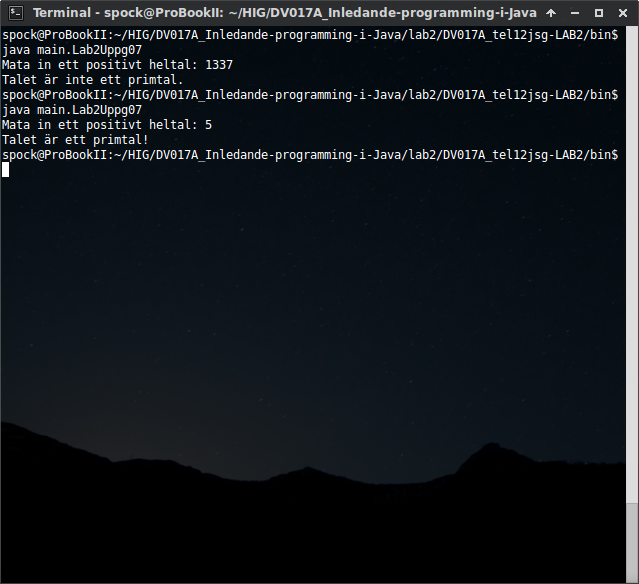
\includegraphics[width=\linewidth]{img/07.png}
    \caption{Körning av koden till Uppgift~\ref{sec:uppg07}}
    \label{fig:uppg07-screenshot}
\end{figure}


%   \section{Uppgift 8}\label{sec:uppg08}

\subsection{Instruktioner}
\begin{verbatim}
8. Skriv en klass Person som innehåller följande instansvariabler, deklarera
   med passande datatyper:

        namn, personnummer, adress, ålder.

   I klassen ska följande metoder ingå:

   * konstruktorn Person, som initierar samtliga instansvariabler.
   * byterNamn, en metod som via parameter ändrar namnet.
   * byterAdress, en metod som via parameter ändrar adressen.
   * fyllerÅr, en metod som lägger till 1 till åldern.
   * hamtaNamn, en metod som returnerar namnet.
   * hamtaPersnr, en metod som returnerar personnumret.
   * hamtaÅlder, en metod som returnerar åldern.
   * hamtaAdress, en metod som returnerar adressen.
   * toString, en metod som i en snyggt formaterad sträng returnerar ett
     Person-objekts *samtliga* data.  Metoden anropas genom att skriva
     objektets (referensens) namn.

   Skriv ett testprogram som testar samtliga metoder i klassen Person.
   Programmet ska i tur och ordning utföra följande:

   * Skapa två Person-objekt, person1 och person2. Den som kör ditt program ska
     mata in startvärden till de båda objektens samtliga data
     (instansvariabler).
   * Skriv ut de båda objektens samtliga data.
   * Låt den som kör ditt program byta namn och adress på person1.
   * Låt person2 fylla år.
   * Skriv ut namnet, personnr och adressen på person1 (skriv alltså inte ut
     åldern).
   * Skriv ut namnet, personnr och åldern på person2 (skriv alltså inte ut
     adressen).
\end{verbatim}


\subsection{Lösning}

\subsubsection{Källkod}
\javacode{src/main/Lab2Uppg08.java}
\caption{Lab2Uppg08.java}
\label{src:uppg08}

\javacode{src/main/Person.java}
\caption{Person.java}
\label{src:Person}


\subsubsection{Skärmdump}
\begin{figure}[htbp]
    \centering
        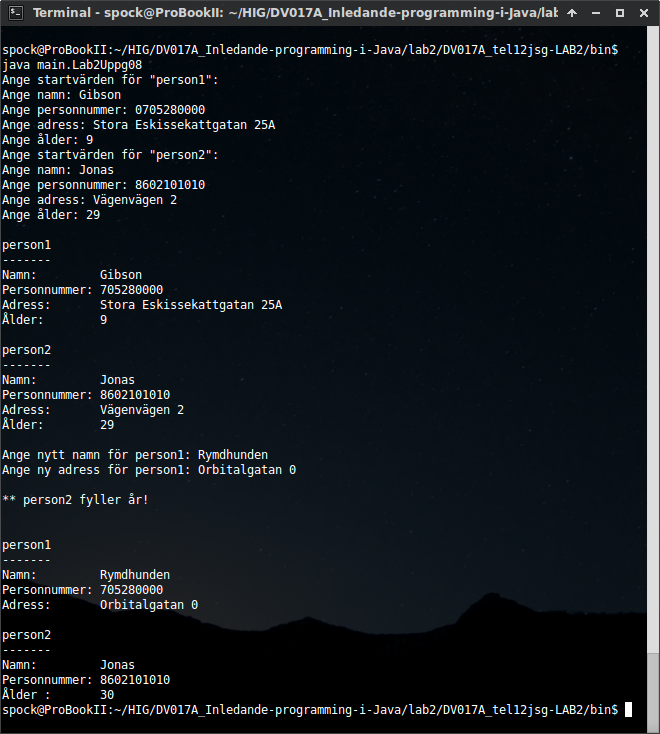
\includegraphics[width=\linewidth]{img/08.png}
    \caption{Körning av koden till Uppgift~\ref{sec:uppg08}}
    \label{fig:uppg08-screenshot}
\end{figure}


%   \section{Uppgift 9}\label{sec:uppg09}

\subsection{Instruktioner}
\begin{verbatim}
9. Skriv en klass Artikel som ska representera ett artikelslag på ett
   varulager. Information som ska finnas om varje artikelslag är:

   artikelnr (int), artikelnamn (String), lagerantal (int), pris
   (double)

   Denna information är alltså klassens instansvariabler, passande datatyp står
   inom parentes. I klassen ska även finnas en *klassvariabel* som håller
   räkning på hur många artikelslag det finns totalt, alltså som innehåller
   totala antalet skapade Artikel-objekt:

   totArtiklar (int)

   I klassen ska följande metoder ingå:

   * konstruktorn Artikel, som initierar samtliga instansvariabler samt
     uppdaterar klassvariabelns värde.
   * ändraNamn, metod som via parameter ändrar på artikelnamnet.
   * hamtaNamn, metod som returnerar artikelnamnet.
   * säljaArtikel, metod som minskar lagerantalet med parameterns värde.
   * fyllaLagret, metod som ökar lagerantalet med parameterns värde.
   * ändraPris, metod som ändrar priset till parameterns värde.
   * hamtaPris, metod som returnerar artikelns pris.
   * hamtaTotAntal, klassmetod som returnerar antalet artikelslag.
   * skrivInfo, metod av returtypen void som skriver ut alla data om en artikel.

   Skriv också ett testprogram, där du testar klassens alla metoder.
\end{verbatim}


\subsection{Källkod}
\javacode{src/main/Lab2Uppg09.java}
\caption{Lab2Uppg09.java}
\label{src:uppg09}

\javacode{src/main/Artikel.java}
\caption{Artikel.java}
\label{src:artikel}


\subsection{Skärmdump}
\begin{figure}[htbp]
    \centering
        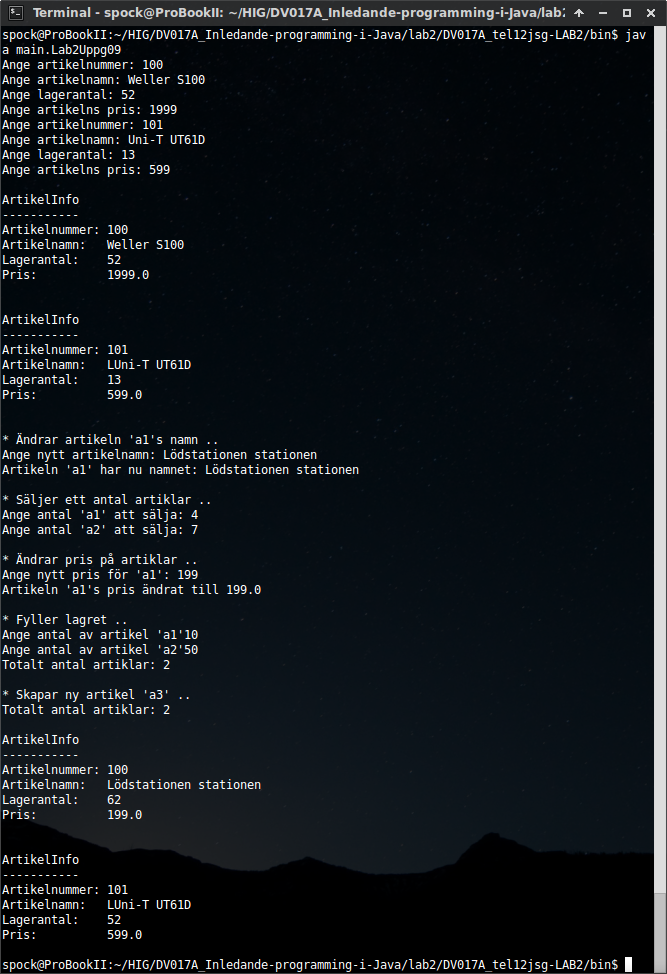
\includegraphics[width=\linewidth]{img/09.png}
    \caption{Körning av koden till Uppgift~\ref{sec:uppg09}}
    \label{fig:uppg09-screenshot}
\end{figure}


    \section{Resultat}\label{sec:resultat}
% TODO: Lägg till resultat och kommentar på hela labben.



    \newpage

    \bibliographystyle{sweplnat}
    \bibliography{tex/referenser}
    \bibliography{referenser}
%   \section{Referenser}\label{sec:ref}

\subsection{Links}\label{sec:links}
% TODO: Lägg till referenser/källor.

\subsection{Source files}\label{sec:source}
% TODO: Eventuell länk till källfiler.



\end{document}
